\subsection{Testing: terminology, types of testing activities}

\definition{Testing} (dynamic analysis) is an approach to verification. The \textbf{main goal of testing is to make programs fail}.

Other \emph{common goals} are:
\begin{itemize}
    \item Exercise different parts of a program to \textbf{increase coverage};
    
    \item Make sure the \textbf{interaction between components works} (\emph{integration testing});
    
    \item Support \textbf{fault localization} and \textbf{error removal} (\emph{debugging});
    
    \item Ensure that \textbf{bugs introduced in the past do not happen again} (\emph{regression testing}).
\end{itemize}
The dynamic analysis \textbf{analyzes program behavior}. The \textbf{properties} are \textbf{encoded as executable oracles representing expected outputs} and \textbf{desired conditions} (assertions).

It can \textbf{run only finite test cases}, so it's not exhaustive verification. The \textbf{failures have concrete inputs that trigger them}, and the \textbf{execution is automatic}.

\begin{flushleft}
    \textcolor{Green3}{\faIcon{question-circle} \textbf{We have often heard about \emph{debugging}, but what is it?}}
\end{flushleft}
\definition{Debugging} is a systematic approach to \textbf{fault localization and error removal}. The output is often used to support debugging.

\begin{figure}[!htp]
    \centering
    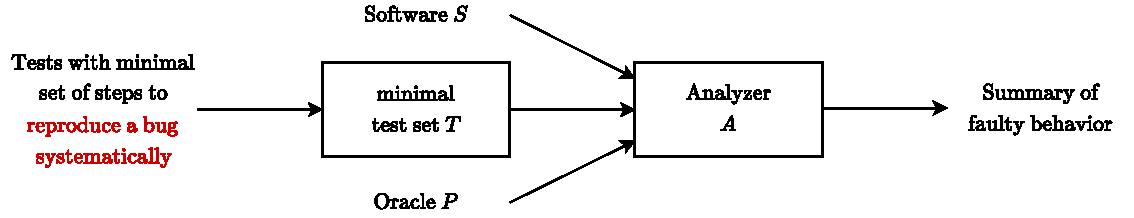
\includegraphics[width=\textwidth]{img/testing-1.pdf}
\end{figure}

\begin{flushleft}
    \textcolor{Green3}{\faIcon{question-circle} \textbf{... and \emph{test case}?}}
\end{flushleft}
\begin{definitionbox}
    A \definition{Test Case} is a set of \textbf{inputs}, \textbf{execution conditions}, and a \textbf{pass/fail criterion}.
\end{definitionbox}

\noindent
Running a test case typically involves setup, execution and teardown.
\begin{itemize}
    \item \textbf{Setup}. Bring the program to an \textbf{initial state} that fulfils the execution conditions.
    
    \item \textbf{Execution}. \textbf{Run} the program on the actual inputs.
    
    \item \textbf{Teardown}. \textbf{Record} the output, the final state, and any \textbf{failure} determined based on the pass/fail criterion.
\end{itemize}
A \textbf{test set}, or \textbf{test suite}, can include \textbf{multiple test cases}. Finally, a \definition{Test Case Specification} is a \textbf{requirement to be satisfied by one or more test cases}. An example of test case specification can be \emph{the input must be a sentence composed of at least two words}, and an example of test case input is \emph{this is a good test case input}.

\highspace
When discussing test cases, it's necessary to introduce \definition{Unit Testing}. This is \textbf{conducted by developers} and \textbf{aims to test small pieces} (units) \textbf{of code in isolation}. 

However, when we test in isolation, there should be a \textbf{problem}: the \textbf{units may depend on other units}. Then, we need to simulate missing units.

\highspace
The \definition{Integration Testing} (integration of the unit tests) \textbf{aims to exercise the interaction between interfaces and components}. The \textbf{faults} discovered by integration testing are multiple; some examples:
\begin{itemize}
    \item \textbf{Inconsistent interpretation of parameters} (e.g. mixed units meters or yards)

    \item \textbf{Violations of assumptions about domains} (e.g. buffer overflow)

    \item \textbf{Side effects on parameters or resources} (e.g. conflict on temporary file)

    \item \textbf{Nonfunctional properties} (e.g. unanticipated performance issues)

    \item \textbf{Concurrency-specific problems}
\end{itemize}
Typically, the integration test is defined by the Design Document. In the Design Document, we can find two types of plans:
\begin{itemize}
    \item \definition{Build Plan} that establishes the \textbf{order of the implementation};
    \item A \definition{Test Plan} that defines how to carry out integration testing is needed.
\end{itemize}
The strategies for the integration test are many:
\begin{itemize}
    \item \definition{Big Bang}: \textbf{test only after integrating all modules} (not even a real strategy). 
    
    \begin{flushleft}
        \textcolor{Green3}{\faIcon{check} \textbf{Pros}}
    \end{flushleft}
    It doesn't require stubs; it only \textbf{requires fewer drivers}/\textbf{oracles}.
    
    \begin{flushleft}
        \textcolor{Red2}{\faIcon{exclamation-triangle} \textbf{Cons}}
    \end{flushleft}
    \begin{enumerate}
        \item Minimum: observability, fault localization/diagnosability, efficacy, feedback;
        \item \textbf{High cost of repair} (cost of repairing a fault increases as a function of time between the introduction of an error in the code and repair).
    \end{enumerate}

    \newpage


    \item \definition{Iterative and incremental strategies}. The main action is \textbf{run after components are released (not just at the end)}. The strategy can be done in three different ways:
    \begin{itemize}
        \item \textbf{Hierarchical}. Based on the hierarchical structure of the system. It can be done top-down or bottom-up.
        \begin{itemize}
            \item \textbf{\emph{Top-down} strategy}. Work \textbf{from the top level} (in terms of \dquotes{use} or \dquotes{include} relationship) \textbf{down to the bottom level}. As modules are completed (according to the building plan), more functionality is testable. We also need to replace some stubs, and we need other stubs for lower levels. \textbf{When all modules are incorporated, the whole functionality can be tested}.
            
            \highspace
            \begin{flushleft}
                \textcolor{Green3}{\faIcon{check} \textbf{Pros}}
            \end{flushleft}
            The drivers use the top level interfaces (e.g. REST APIs).
            
            \highspace
            \begin{flushleft}
                \textcolor{Red2}{\faIcon{exclamation-triangle} \textbf{Cons}}
            \end{flushleft}
            This strategy requires stubs of used modules at each step of the process.

            \begin{figure}[!htp]
                \centering
                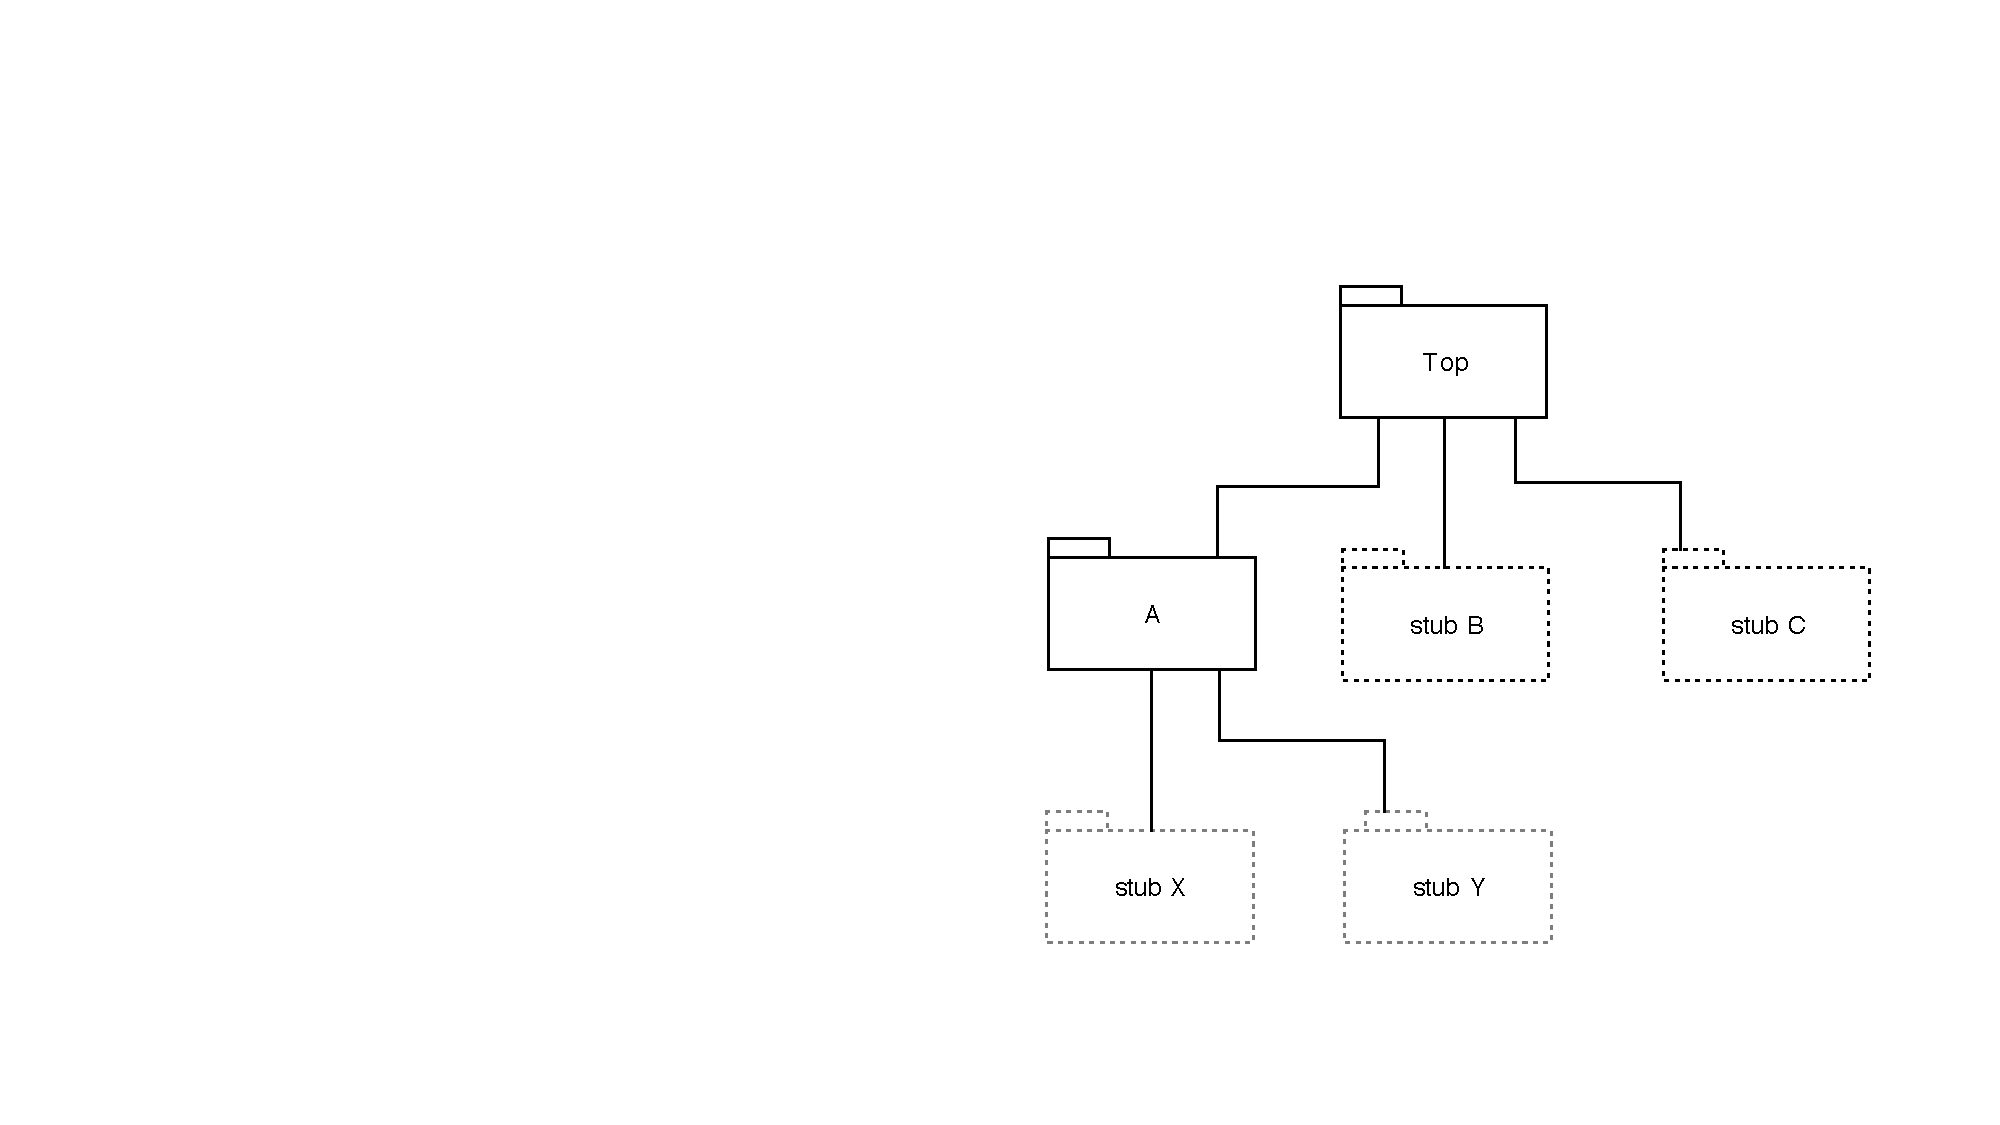
\includegraphics[width=.6\textwidth]{img/top-down-1.pdf}
                \caption{\example{Example} of top-down strategy.}
            \end{figure}
            
            \newpage

            \item \textbf{\emph{Bottom-up} strategy}. Starting from the leaves of the \dquotes{uses} hierarchy. 
            
            \highspace
            \begin{flushleft}
                \textcolor{Green3}{\faIcon{check} \textbf{Pros}}
            \end{flushleft}
            An advantage is that it \textbf{doesn't require stubs}.
            
            \highspace
            \begin{flushleft}
                \textcolor{Red2}{\faIcon{exclamation-triangle} \textbf{Cons}}
            \end{flushleft}
            \textbf{Typically requires more drivers} (one for each module, as in unit testing). Can this be a disadvantage? Maybe, because the newly developed module may replace an existing driver, and new modules require new drivers.

            Another thing to consider is that \textbf{it may create several working subsystems}, and each working subsystem will eventually be integrated into the final one.

            \begin{figure}[!htp]
                \centering
                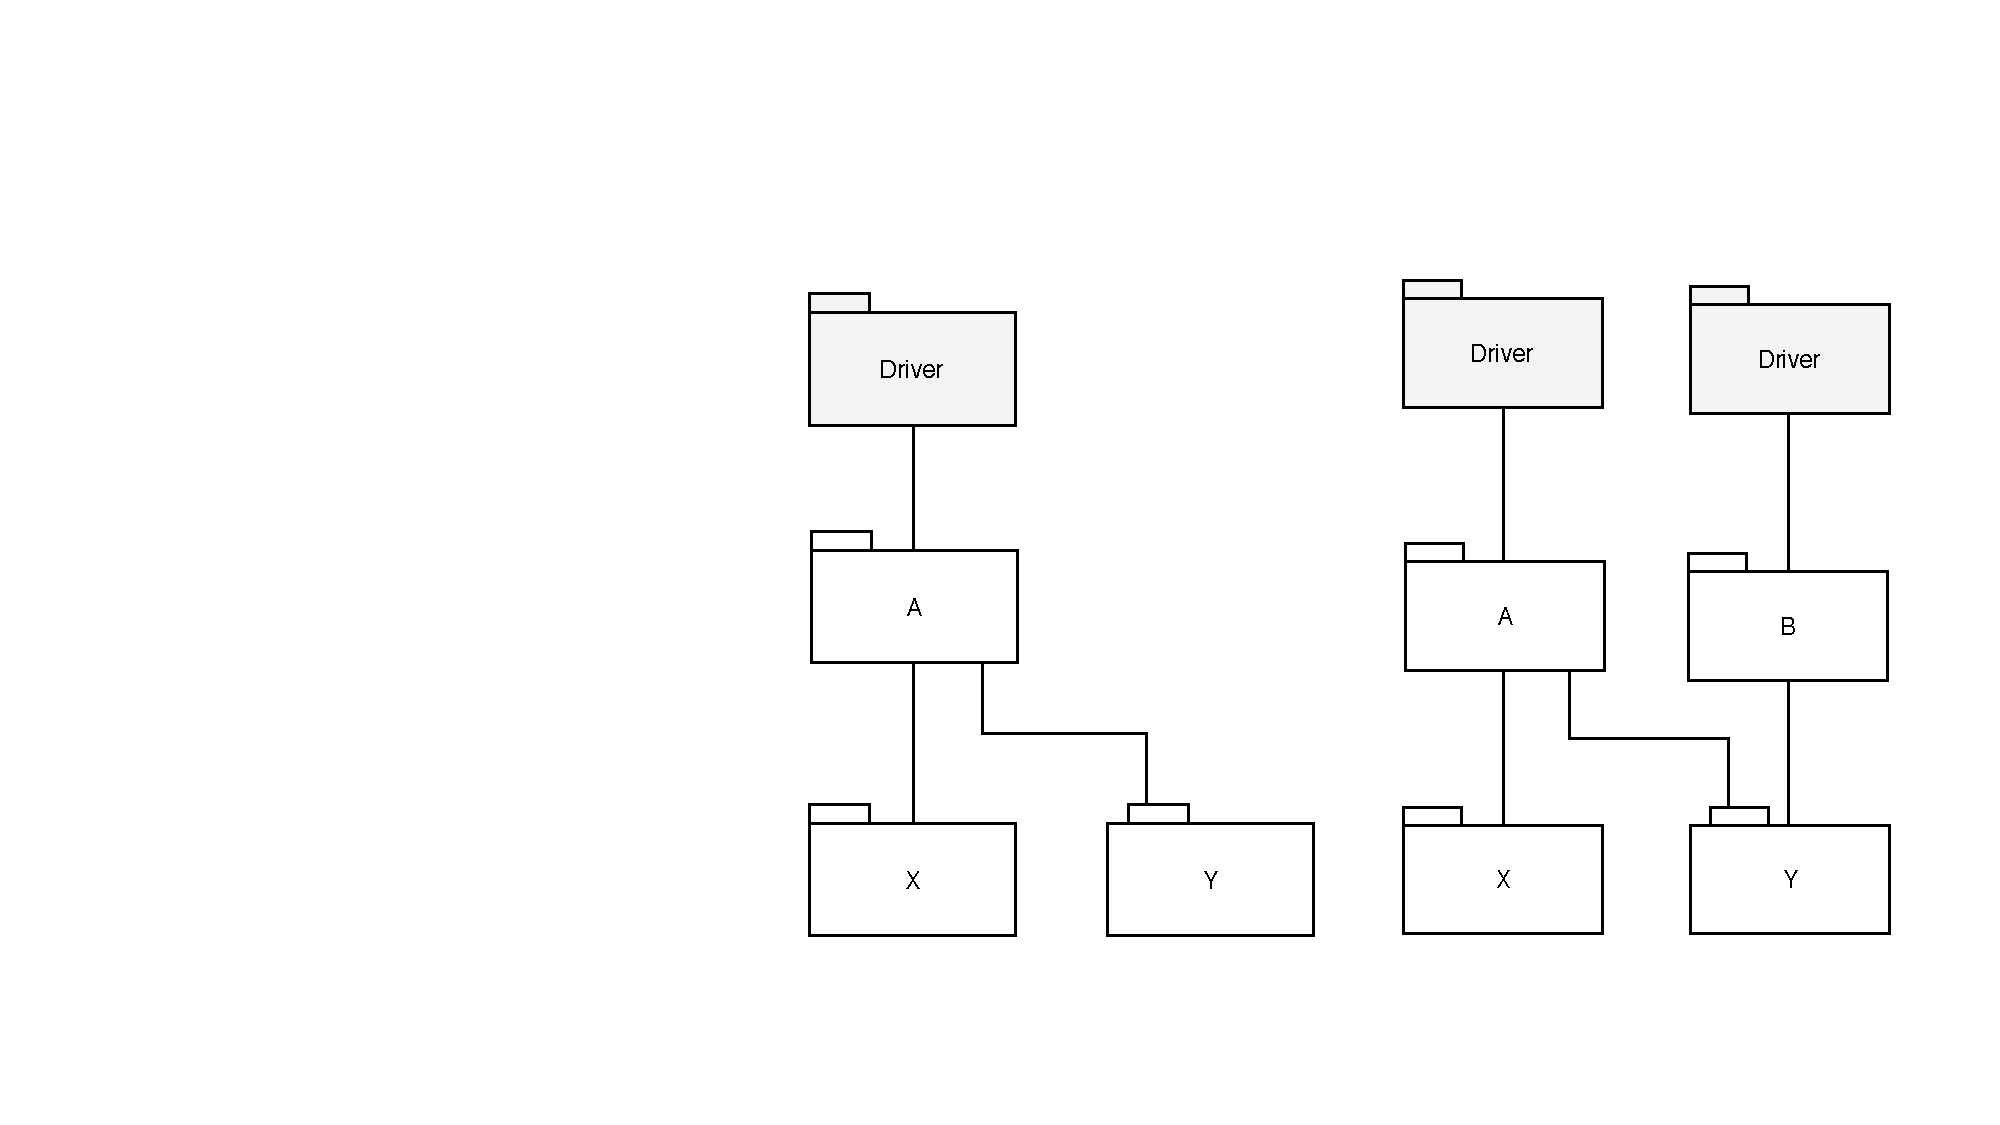
\includegraphics[width=.6\textwidth]{img/bottom-up-1.pdf}
                \caption{\example{Example} of bottom-up strategy.}
            \end{figure}
        \end{itemize}

        \newpage

        \item \textbf{Threads}. A \textbf{thread is a part of several modules that together provide a user-visible programme function}. By using the thread strategy we can have some \textbf{advantages}.
        \begin{flushleft}
            \textcolor{Green3}{\faIcon{check} \textbf{Pros}}
        \end{flushleft}
        \begin{itemize}
            \item We can \textbf{maximize the progress visible to the user} (or other stakeholders);
            \item \textbf{Reduce drivers and stubs};
            \item An integration plan is usually more complex.
        \end{itemize}
        \begin{figure}[!htp]
            \centering
            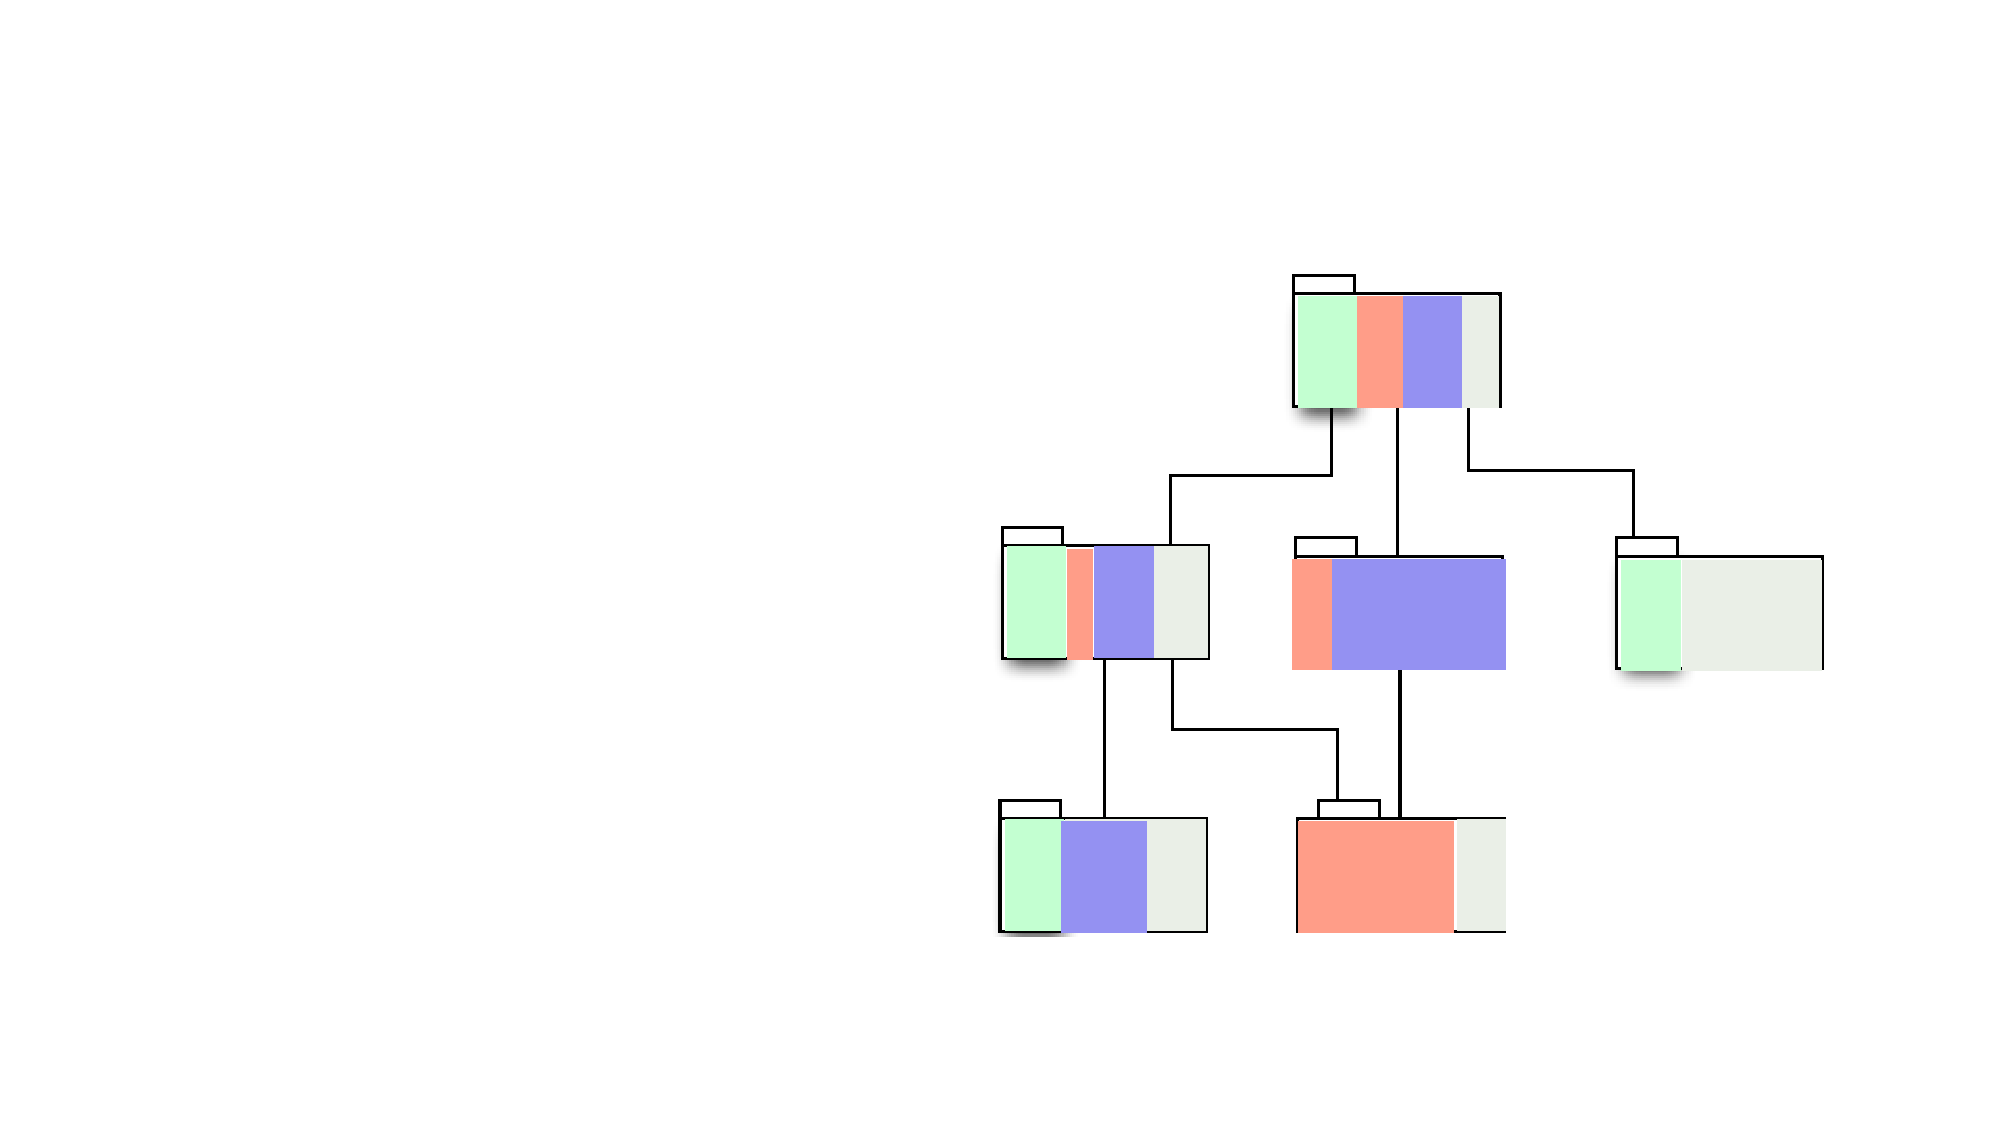
\includegraphics[width=.6\textwidth]{img/threads-1.pdf}
            \caption{\example{Example} of threads strategy.}
        \end{figure}
        
        \item \textbf{Critical}. The critical modules strategy \textbf{starts with the highest risk modules}. Risk assessment is a necessary first step. It can include technical risks (e.g. is X feasible?) and process risks (e.g. is the schedule for X realistic?). It may also be similar to a priority process.

        The \textbf{key point of this strategy is the risk-oriented process}. Integration and testing as a risk mitigation activity, designed to \emph{deliver any bad news as early as possible}.
    \end{itemize}
\end{itemize}

\begin{flushleft}
    \textcolor{Green3}{\faIcon{question-circle} \textbf{Which one should we choose?}}
\end{flushleft}
Given the three strategies above, \emph{which one should we choose}? Well, the structural strategies (bottom-up or top-down) are simpler, but thread and critical modules provide better external visibility of progress (especially in complex systems).

\highspace
So the \textbf{best choice} should be a \textbf{combination of different strategies}:
- Use \textbf{top-down/bottom-up} for relatively \textbf{small components} and \textbf{subsystems};
- Combinations of \textbf{thread} and \textbf{critical module integration testing} for \textbf{larger subsystems}.

\newpage

\subsubsection{E2E Testing}

\begin{definitionbox}
    \definition{End-to-end (E2E)} testing is a \textbf{software testing methodology to test a functional and data application flow consisting of several sub-systems working together from start to end}.\footnote{\href{https://microsoft.github.io/code-with-engineering-playbook/automated-testing/e2e-testing/}{Engineering Fundamentals Playbook}}
\end{definitionbox}

\noindent
At times, these systems are developed in different technologies by different teams or organizations. Finally, they come together to form a functional business application. Hence, testing a single system would not suffice. Therefore, end-to-end testing verifies the application from start to end putting all its components together.

\highspace
The following is a list of \textbf{common types of tests} that use the E2E system:
\begin{itemize}
    \item \definition{Functional Testing}
    \begin{flushleft}
        \textcolor{Red2}{\faIcon{book} \textbf{Purpose}}
    \end{flushleft}
    Check whether the \textbf{software meets the functional requirements}.

    \begin{flushleft}
        \textcolor{Green3}{\faIcon{question-circle} \textbf{How?}}
    \end{flushleft}
    Use the software as described by use cases in the RASD (pag. \pageref{RASD}), check whether requirements are fulfilled.


    \item \definition{Performance Testing}
    \begin{flushleft}
        \textcolor{Red2}{\faIcon{book} \textbf{Purpose}}
    \end{flushleft}
    \begin{enumerate}
        \item Detect \textbf{bottlenecks} affecting response time, utilization, throughput
        \item Detect \textbf{inefficient algorithms}
        \item Detect \textbf{hardware/network issues}
        \item Identify \textbf{optimization possibilities}
    \end{enumerate}

    \begin{flushleft}
        \textcolor{Green3}{\faIcon{question-circle} \textbf{How?}}
    \end{flushleft}
    Load the system with the expected workload and measure and compare acceptable performance.
    
    \newpage

    \item \definition{Load Testing}
    \begin{flushleft}
        \textcolor{Red2}{\faIcon{book} \textbf{Purpose}}
    \end{flushleft}
    \begin{enumerate}
        \item \textbf{Expose bugs} such as memory leaks, mismanagement of memory, buffer overflows
        \item Identify \textbf{upper limits of components}
        \item \textbf{Compare alternative architectural options}
    \end{enumerate}

    \begin{flushleft}
        \textcolor{Green3}{\faIcon{question-circle} \textbf{How?}}
    \end{flushleft}
    Test the system at increasing workload until it can support it, and load the system for a long period.


    \item \definition{Stress Testing}
    \begin{flushleft}
        \textcolor{Red2}{\faIcon{book} \textbf{Purpose}}
    \end{flushleft}
    Make sure that the \textbf{system recovers gracefully after failure}.

    \begin{flushleft}
        \textcolor{Green3}{\faIcon{question-circle} \textbf{How?}}
    \end{flushleft}
    Trying to break the system under the test by overwhelming its resources or by reducing resources.

    For \example{example} double the baseline number for concurrent users/HTTP connections, or randomly shut down and restart ports on the network switches/routers that connect servers.
\end{itemize}